\subsubsection{Introduction}

Part e aims to combine the previous sections, applying a combination of dropout,
data augmentation and batch normalization to the baseline model from Part a.
The aim is to develop a CNN with the optimal accuracy.

\subsubsection{Rational}

By combining the advantages of the techniques used in the previous sections,
a CNN can be developed which outperforms the baseline model developed in Part a.
While it is not necessary to utilise all of the techniques, combinations of data
augmentation, dropout, and batch normalisation can lead to improved accuracy
for the neural network.

\subsubsection{Design}

The design of this section came about from the combination of the techniques in
each of the previous sections. As discussed in the Testing section below,
different combinations of the techniques were tested in order to obtain the best
possible accuracy from the model. The final code for this section can be seen in
the appendices.

\begin{figure}[H]
	\centering
	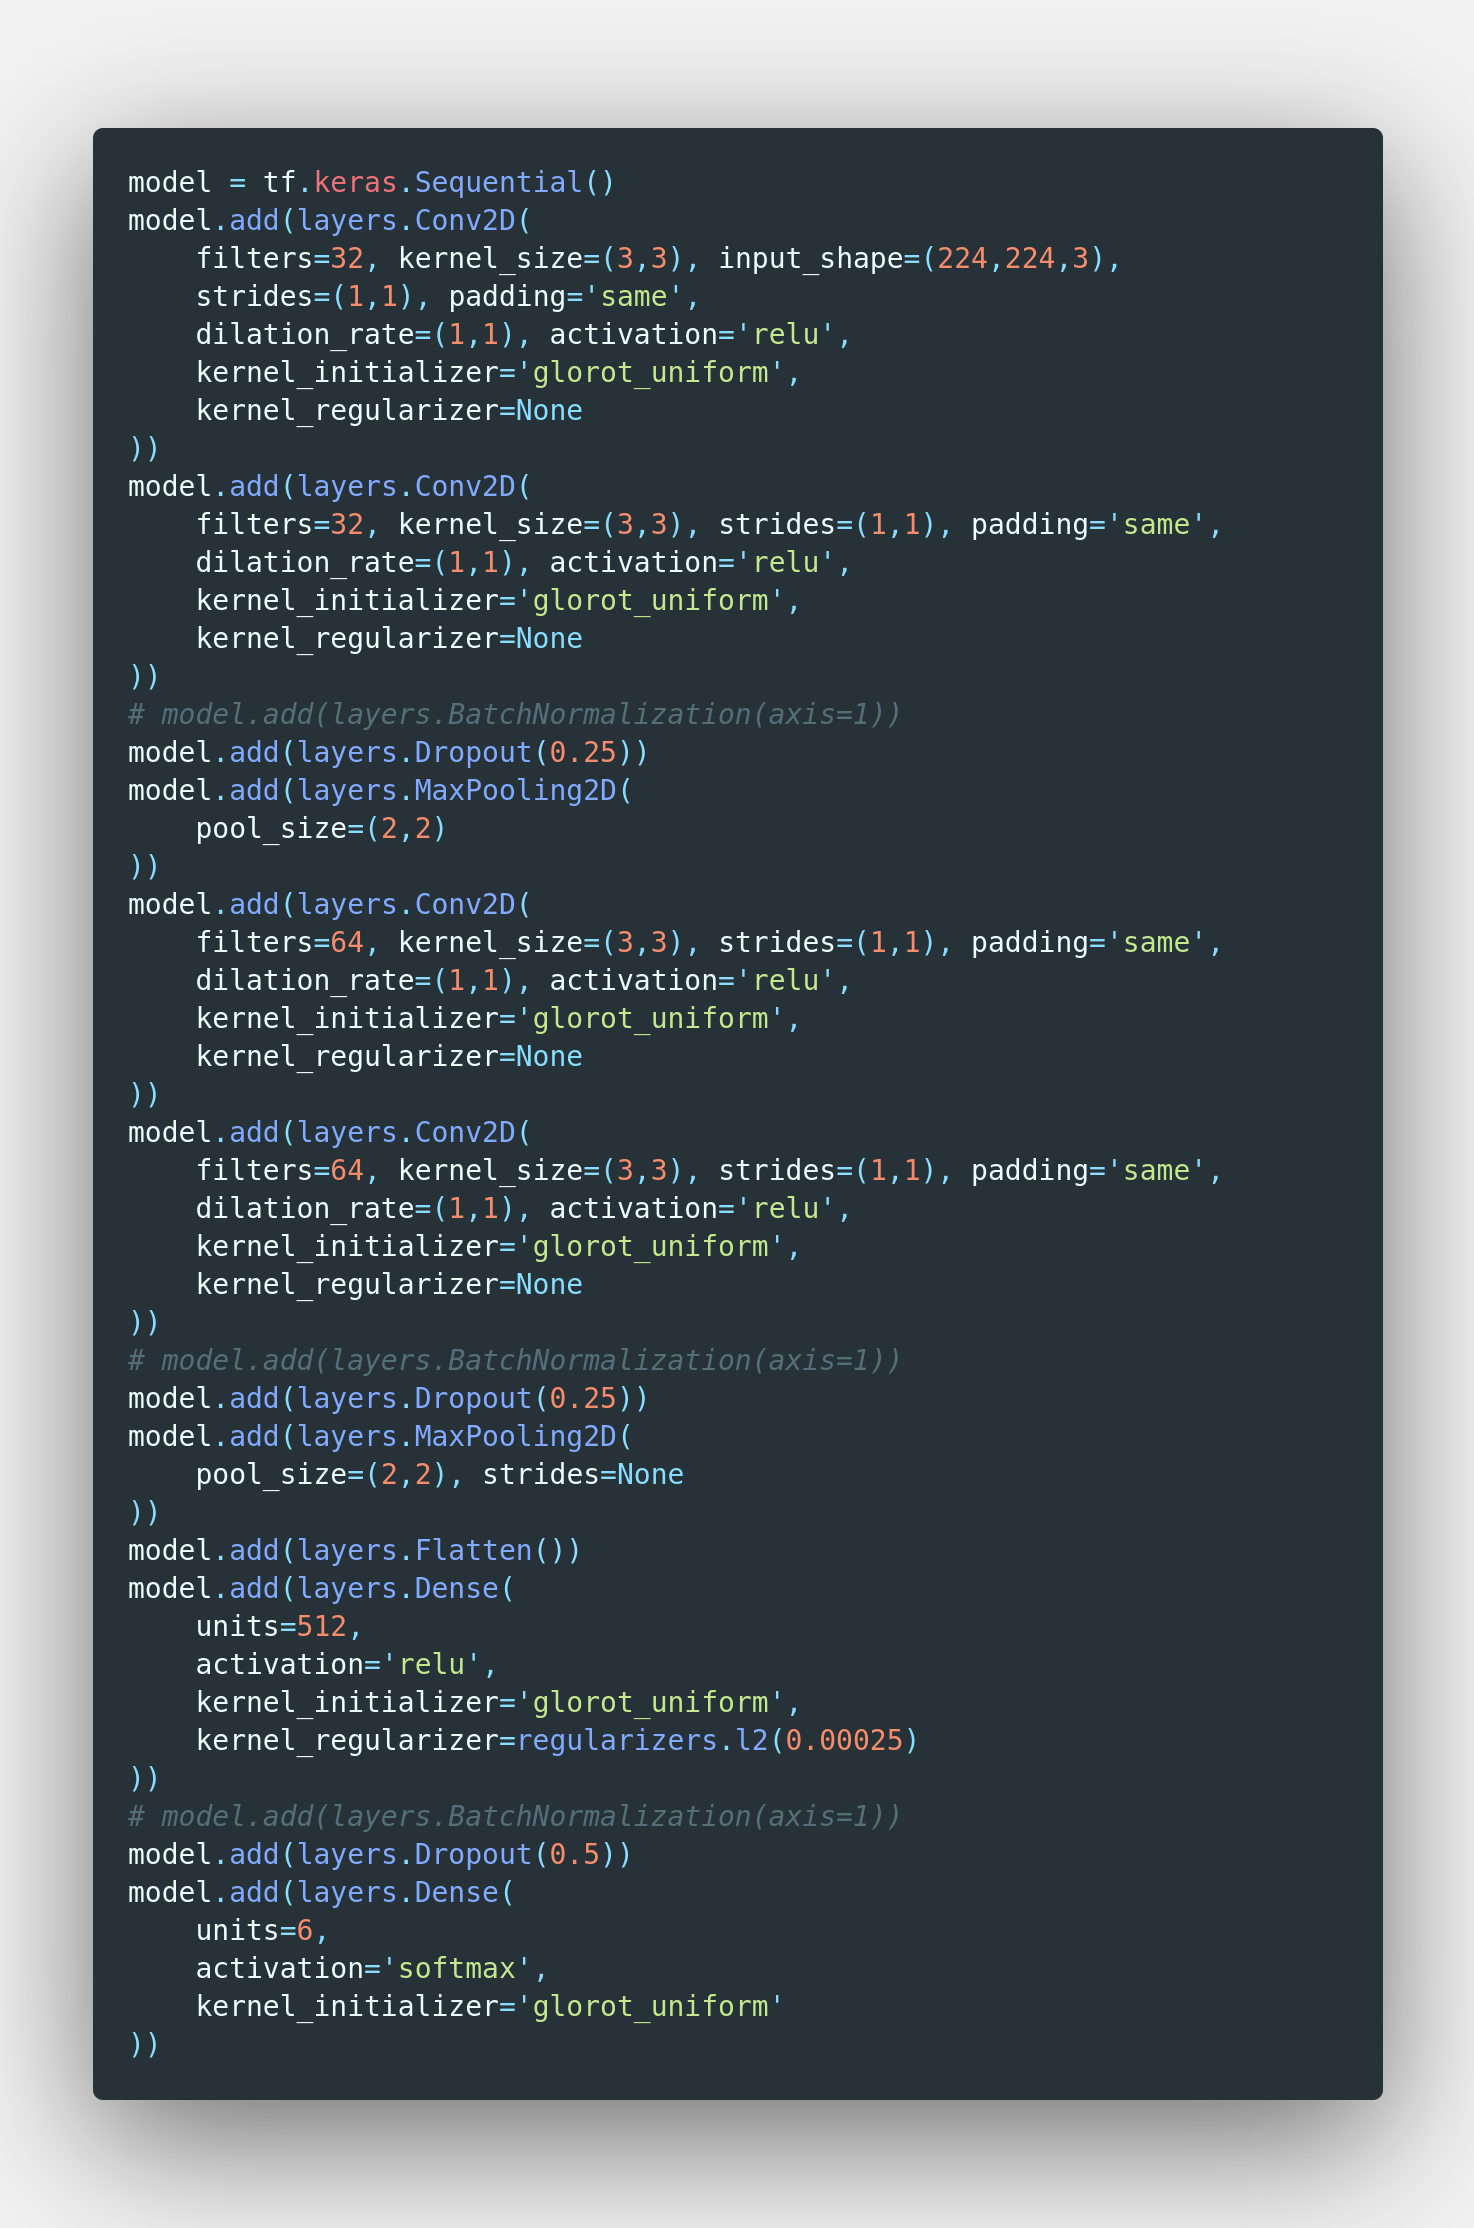
\includegraphics[width=0.8\textwidth]{images/Code/combo}
	\caption{Combined Technique Model}
	\label{fig:images-Code-combo}
\end{figure}

\subsubsection{Testing}

Testing was again done manually, and as such, the obtained result is suboptimal.

\begin{table}[H]
	\centering
	\caption{Layer and HyperParameter Testing}
	\label{tab:q1pe}
	\begin{tabular}{|c|c|}
	\hline
	CNN Description & Validation Accuracy \\
	\hline
	Combined Part a-d & 76.17 \\
	Batch Normalisation + Data Augmentation & 76.17 \\
	Dropout + Data Augmentation & 71.17 \\
	Batch Normalisation + Dropout & 70.5 \\
	No Batch Normalisation in the output layers & 72.5 \\
	No Dropout in the output layers & 66.2 \\
	\hline
	\end{tabular}
\end{table}

By using only Dropout and Data Augmentation , and a dropout rate of 0.25 for
the non-output
Dropout layers, a highest validation accuracy of 78.17\% was achieved. This is
far from optimal, however it is approximately on par with the results obtained
from using Dropout and Data Augmentation separately. This is undoubtably due to
poor hyperparameter tuning.

\subsubsection{Results}

The model summary shown below displays the use of dropout within the model. As
mentioned, data augmentation was also applied to the input images in order to
achieve the performance that is seen in the results.

\begin{figure}[H]
	\centering
	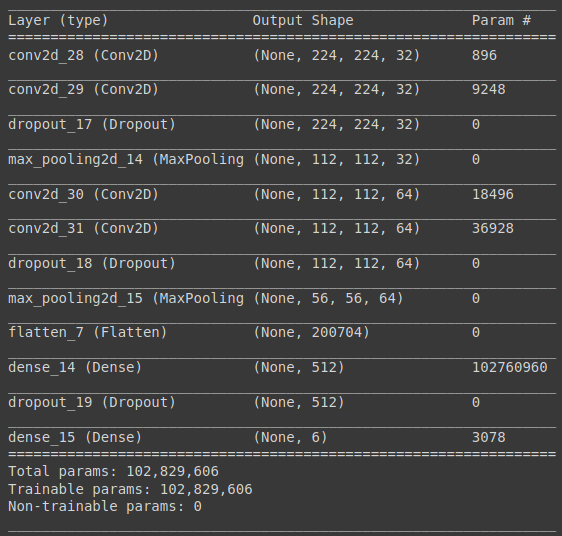
\includegraphics[width=0.8\textwidth]{images/q1/pe/q1pemodel}
	\caption{Model Summary}
	\label{fig:q1pemodel}
\end{figure}

The model seems to be overfitting to the training set. This is an issue as the
training set does not have extremely high accuracy, and this is likely causing
issues with the predictions of the test set.

While the loss is relatively low, the overall accuracy does not benefit from
this improvement in the system.

\begin{figure}[H]
	\centering
	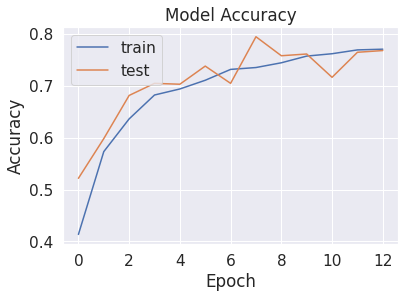
\includegraphics[width=0.8\textwidth]{images/q1/pe/accuracy}
	\caption{Validation and Training Accuracy}
	\label{fig:q1peacc}
\end{figure}


\begin{figure}[H]
	\centering
	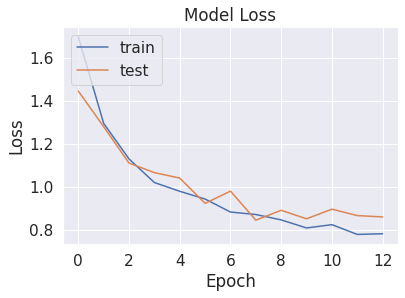
\includegraphics[width=0.8\textwidth]{images/q1/pe/loss}
	\caption{Validation and Training Loss}
	\label{fig:q1peloss}
\end{figure}

The test results can be seen in Figure \ref{fig:q1peresults}. The average
precision is 82\%, while the average recall is 82\%. These values are below the
values achieved using only Data Augmentation techniques. Again, this is likely
due to the poor implementation of hyperparameter tuning, i.e. trial-and-error.

\begin{figure}[H]
	\centering
	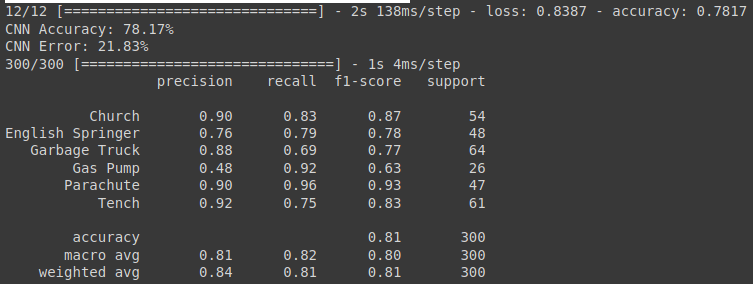
\includegraphics[width=0.8\textwidth]{images/q1/pe/results}
	\caption{Model Testing Results}
	\label{fig:q1peresults}
\end{figure}

The confusion matrix in Figure \ref{fig:q1pematrix} shows that the highest
number of correctly identified samples belonged to the ``Church'' class.

\begin{figure}[H]
	\centering
	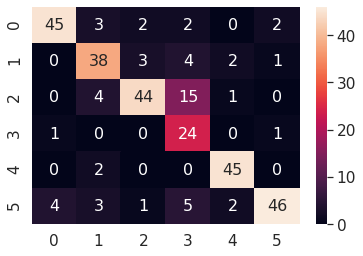
\includegraphics[width=0.8\textwidth]{images/q1/pe/matrix}
	\caption{Confusion Matrix}
	\label{fig:q1pematrix}
\end{figure}

The training time of this model was 1138.7972 seconds, which is 4.745lbs of CO2
equivalent emissions.
